\documentclass[11pt, oneside]{article}   	% use "amsart" instead of "article" for AMSLaTeX format
\usepackage{geometry}                		% See geometry.pdf to learn the layout options. There are lots.
\geometry{letterpaper}                   		% ... or a4paper or a5paper or ... 
%\geometry{landscape}                		% Activate for for rotated page geometry
%\usepackage[parfill]{parskip}    		% Activate to begin paragraphs with an empty line rather than an indent
\usepackage{graphicx}				% Use pdf, png, jpg, or eps� with pdflatex; use eps in DVI mode
								% TeX will automatically convert eps --> pdf in pdflatex		
\usepackage{amssymb}
\graphicspath{{/Users/telliott_admin/Dropbox/Tex/png/}}
\usepackage{parskip}

\title{Area of a circle by integration}
%\author{The Author}
\date{}							% Activate to display a given date or no date

\begin{document}
\maketitle
%\section{}
%\subsection{}
\noindent

\begin{center}
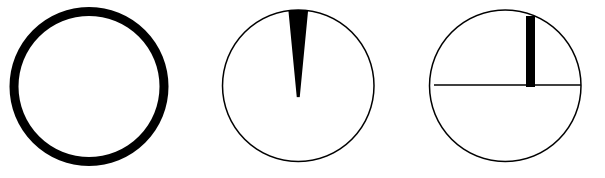
\includegraphics [scale=0.5] {circles.png}
\end{center}
\large
Integration is used to compute areas and volumes, and other sums, by adding up many little pieces.  To calculate the area of a circle, we find the pieces we will use with one of three basic strategies:  rings, slices of pie, and rectangles of area underneath the function obtained by solving $x^2 + y^2 = R^2$, and using the positive square root.  These three approaches are illustrated in the figure above.

\subsection*{Rings}

In the first approach (left panel), we imagine the area being computed by adding up the individual areas of a series of very thin, concentric rings.

The total area to be computed is that of a circle of a definite, fixed size, and we denote the radius of this circle by capital $R$, a constant.  On the other hand, the series of rings ranges from the origin of the circle to the circumference of the outmost ring.  Each one of this progression of rings has a radius, so we use the lowercase $r$ to describe them, with $r$ being a variable---$r$ varies from $0$ at the origin to $R$ at the outside of the circle.

Think about an individual ring, for example the outermost ring, which is similar to the peel or rind surrounding a slice of lemon.  We are working with areas here, in two dimensions, so the slice we imagine to be infinitely thin, and we are working with it as a cross-section or ring.  The area of the ring is the length times the width.  The length is the circumference, $2 \pi R$ for the outermost ring, but in general, for any of the inner rings it is $2 \pi r$. The length is multiplied by the width of the slice, which is a small element of radius, $dr$.  The small element of area contributed by an individual ring is $dA$:

\[ dA = 2 \pi r \ dr \]

Another way to explain this equation is to ask the question:  \emph{how does area change with increasing radius}?  If we take a circle and increase its radius by a bit, how does the area change?  The answer is, it changes in proportion to the circumference, $2 \pi r$.

Proceeding from the equation, the total area is the sum of the areas for the series of rings.

\[ A = \int dA = \int_0^R 2 \pi r \ dr \]

It's worth emphasizing how this view is much different than our first uses of integration:  the pieces of area are no longer rectangles but circles.  But it poses most clearly the question we are trying to answer, "how does area vary with $r$"?

The solution is
\[ \int_0^R 2 \pi r \ dr = 2 \pi \ \frac{1}{2}r^2 \ \bigg|_{r=0}^{r=R} = \pi R^2\]

\subsection*{Wedges}

In the second method, we need to first find the area of a wedge.  For a thin enough slice, this is a triangle, with a similar formula: one-half the base times the height.  The height is $R$, the radius of the circle.  

For the base we need the length of a piece of arc of a circle.  Recall that by definition, if we have a unit circle, then the angle of a wedge is equal to the arc it cuts out, and vice-versa, the arc is equal to the angle.  (Thus, the total length if we go all the way around the unit circle is $2 \pi$).  For a circle with radius $R$, the length going all the way around is $2 \pi R$, and the length of arc for any angle $\theta$ is $\theta$ times $R$.

Our area is built up of a series of wedges that are almost infinitely slender, with angle $d \theta$, so these wedges have bases measuring $R \ d \theta$.  The area of each wedge is

\[ dA = \frac{1}{2} R \ R \ d\theta \]

And we have for the total area
\[ A = \int dA = \int  \frac{1}{2} R \ R \ d\theta \]
\[= \frac{1}{2} R^2 \int_{\theta=0}^{\theta=2\pi} \ d\theta \]
\[ = \frac{1}{2} R^2 \theta \  \bigg|_{\theta=0}^{\theta=2\pi} \]
\[ =  \pi R^2 \]

\subsection*{Area under the curve}

The third view is the most familiar, but has a substantially harder calculation.  We need to find the area under the positive square root in the equation for a circle, between some limits, which could be $x=0  \Rightarrow x=R$ or $x=-R  \Rightarrow x=R$ .

\[ x^2 + y^2 = R^2\]
\[ y = \sqrt{R^2-x^2} \] 
We use a trigonometric substitution
\[ x = R \sin \theta \]
\[ y = R \cos \theta \]
\[ dx = R \cos \theta \ d\theta \]
The integral we want to calculate is:
\[ \int \sqrt{R^2 - x^2} \ dx \]

We \emph{could} substitute $x=R \sin \theta$:
\[ \sqrt{R^2 - x^2} \]
\[ =  \sqrt{R^2 - R^2 \sin^2 \theta} \]
\[ = R \sqrt{1 - \sin^2 \theta} \]
\[ = R \sqrt{\cos^2 \theta} \]
\[ = R \cos \theta \]
plugging in for $dx$ we obtain:
\[ = \int R \cos \theta \ R \cos \theta \ d\theta \]
\[ = \int R^2 \cos^2 \theta \ d\theta \]

Alternatively, just recognize that we want to integrate value of $y$
\[ \int y \ dx \]
\[ = \int R \cos \theta \ R \ cos \  \theta \ d\theta \]
\[ = R^2 \int \cos^2 \theta \ d\theta \]
We have worked this integral out elsewhere (or you can solve it by substituting from the double angle formula).  We obtain 
\[ R^2 \int \cos^2 \theta \ d\theta = \frac{1}{2}R^2 \int (1 + \cos \ 2\theta) \ d \theta \]
\[ =  \frac{1}{2}R^2  \ [ \ \theta +   \frac{1}{2} \sin \ 2 \theta \ ]  \]

\subsection*{Area under the curve:  limits}

To actually compute the are, we need limits.  Suppose we take the limits for the original integral as 
\[ x = 0, \ \ \ \  x = R \]
and agree that we need to multiply the final result by $4$, because we're calculating only the upper-right quarter of the circle. 

After the substitution of $\theta$ for $x$, these limits become

\[ x = 0 = R \sin \theta, \ \ \ \  \theta =  \frac{ \pi}{2} \]
\[ x = R = R \sin \theta, \ \ \ \  \theta = 0 \]

But there's a subtlety lurking here.  If we integrate from $\theta > 0$ to $\theta = 0$, the area will be negative.  To fix this, we must reverse the order of the limits.  

With an upper limit equal to $\pi/2$, and 0 as the lower limit, the term in brackets is
\[ (\frac{\pi}{2}  + \frac{1}{2} \sin \ \pi) - (0 + \frac{1}{2} \sin 0) = \frac{\pi}{2} \]
\[ A = \frac{1}{4} \pi R^2    \]
This is one-fourth of the total, hence $A_{T} =\pi R^2$.
\end{document}  